\documentclass[a4paper,10pt]{ltjsarticle}

% プリアンブル
\usepackage{graphicx}
\usepackage{color}
\usepackage{amsthm}
\usepackage{amsmath}
\usepackage{amsfonts}
\usepackage{mathtools}
\usepackage{listings}
\usepackage[dvipdfmx]{hyperref}
\usepackage{here}
\usepackage{amssymb}
\usepackage{algorithmic}
\usepackage{algorithm}
\usepackage{bbm}
\usepackage{caption}
\usepackage{fancyhdr}
\pagestyle{fancy}
\rhead{Survey by D. Nishiyama on \today}    % ヘッダの右側
\cfoot{\thepage}                % フッター中央
\renewcommand{\headrulewidth}{0pt}        % ヘッダの線の太さ:0ptで消える

\newcommand{\bi}[1]{\ensuremath{\boldsymbol{#1}}}
\newcommand{\propose}{Class-Sensitive}
\newcommand{\multicell}[2]{\begin{tabular}{c}
                               #1\\#2
\end{tabular}}


% 転置記号
\newcommand{\T}{\ensuremath{^{\text{T}}}}

% 図の参照
\newcommand{\Zu}[1]{図\ref{fig:#1}}

% 表の参照
\newcommand{\Hyou}[1]{表\ref{tab:#1}}
\newcommand{\II}{I\hspace{-.1em}I}
% 式の参照
\newcommand{\Shiki}[1]{式\eqref{eq:#1}}
\newcommand{\1}{\mbox{1}\hspace{-0.25em}\mbox{l}}
\lstset{
    basicstyle={\ttfamily\small}, %書体の指定
    frame=tRBl, %フレームの指定
    framesep=10pt, %フレームと中身(コード)の間隔
    breaklines=true, %行が長くなった場合の改行
    linewidth=15cm, %フレームの横幅
    lineskip=-0.5ex, %行間の調整
    tabsize=2 %Tabを何文字幅にするかの指定
}
\usepackage{multirow}
\usepackage{stmaryrd}
\usepackage{subfiles}
\theoremstyle{definition}
\newtheorem{theorem}{定理}
\newtheorem*{theorem*}{定理}
\newtheorem{prop}{命題}
\newtheorem*{prop*}{命題}
\newtheorem{definition}[theorem]{定義}
\newtheorem*{definition*}{定義}

\def\hlineb{%
    \noalign{\ifnum0=`}\fi\hrule \@height \arrayrulewidthb \futurelet
    \reserved@a\@xhlineb}
\def\@xhlineb{\ifx\reserved@a\hlineb
\vskip\doublerulesep
\vskip-\arrayrulewidthb
\fi
\ifnum0=`{\fi}}

\newcommand{\argmax}{\mathop{\rm arg~max}\limits}
\newcommand{\argmin}{\mathop{\rm arg~min}\limits}

%!  心構え
%!  ・時間を決めて読む
%!  ・まとめる癖をつける


%! 読む順番 パターンA(じっくり)
%!  1.アブストラクト(何をしたか)、イントロダクション(何をしたいか)
%!  2.結論(何をしたか・詳細)
%!  3.実験結果(主張の証明)・議論(良し悪し)
%!  4.関連研究(他との違い)、メソッド(実験方法)

%! 読む順番 パターンB(ざっくり)
%!  1.アブストラクト(何をしたか)
%!  2.イントロダクション(何をしたいか)
%!  3.結果(主として図)
\title{GNNExplainer: Generating Explanations for Graph Neural Networks\cite{ying2019gnnexplainer}}
\author{Zhitao Ying, Dylan Bourgeois, Jiaxuan You, Marinka Zitnik, Jure Leskovec}
\date{2019 NeurIPS}
% Document
\begin{document}
    \maketitle
    \abstract{
        グラフニューラルネットワーク(GNN)は、グラフ上の機械学習のための強力なツールである。
        GNNは入力グラフのエッジに沿って再帰的にニューラルメッセージを渡すことにより、
        ノードの特徴情報とグラフ構造を結合する。
        しかし、グラフ構造と特徴情報の両方を取り込むと複雑なモデルになり、
        GNNによる予測を説明することは未解決である。本論文では、GNNEXPLAINERを提案する。
        これは、あらゆるグラフベースの機械学習タスクにおいて、あらゆるGNNベースのモデルの予測に対して、
        相互に予測可能な説明を提供する、初の一般的でモデルにとらわれないアプローチである。GNNEXPLAINERは
        、GNNの予測に重要な役割を持つコンパクトな部分グラフ構造とノード特徴の小さなサブセットを特定する。さらに、
        GNNEXPLAINERはインスタンスのクラス全体に対して一貫性のある簡潔な説明を生成することができる。我々はGNNEXPLAINERを、
        GNNの予測と可能な部分グラフ構造の分布との間の相互情報を最大化する最適化タスクとして定式化する。合成グラフと実グラフを用いた実験により、
        我々のアプローチはノードの特徴だけでなく、重要なグラフ構造も特定できることが示され、
        説明精度において代替ベースラインアプローチを最大43.0\%上回ることが示された。
        GNNEXPLAINERは、意味的に関連する構造を可視化する能力から、解釈可能性、欠陥のあるGNNのエラーに対する洞察に至るまで、様々な利益を提供する。
    }


    \section{どういう論文?}
    \cite{li2022explainability}: 「GNNExplainerは重要でないエッジ/ノードの特徴をマスクすることでGNNを説明することを提案した.具体的には、GNNExplainer は、個々のサンプルごとに入力グラフの学習可能なマスクを学習する。」
    \begin{itemize}
        \item GNNの予測を説明するためのアプローチであるGNNEXPLAINERを提案
        \item 重要なサブグラフがGNNの予測との相互情報量を最大化するように最適化する
        \item 重要でないエッジとノードがマスクされ、予測に重要なサブグラフが強調される
        \item GNNのための最初の説明手法であると主張
    \end{itemize}
    そもそものGNNの説明が簡潔でわかりやすかった
    \begin{figure}[H]
        \centering
        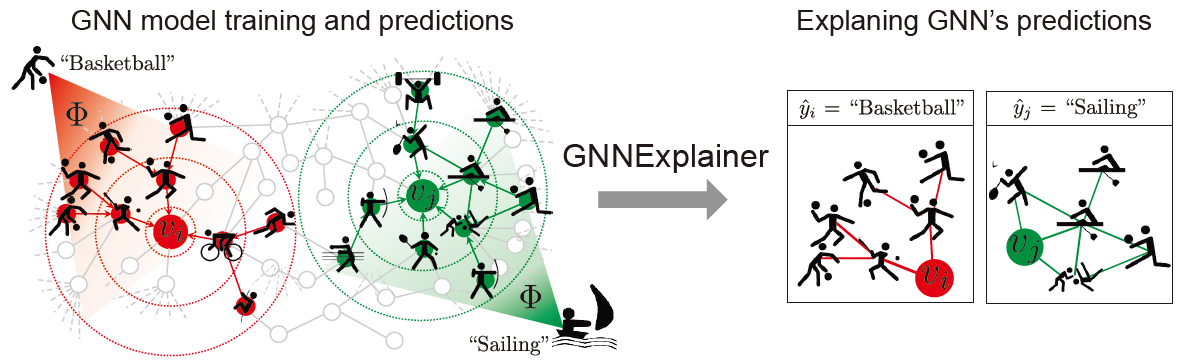
\includegraphics[width=120mm]{fig/gnnexplainer_fig1}
        \caption{
            GNNEXPLAINER provides interpretable explanations for predictions made by any GNN model on
            any graph-based machine learning task. Shown is a hypothetical node classification task where
            a GNN model $\Phi$ is trained on a social interaction graph to predict future sport activities.
            Given a trained GNN $\Phi$ and a prediction $\hat{y}_{i}$ $=$ "Basketball" for person $v_{i}$,
            GNNEXPLAINER generates an explanation by identifying a small subgraph of the input graph together
            with a small subset of node features (shown on the right) that are most influential for $\hat{y}_{i}$.
            Examining explanation for $\hat{y}_{i}$, we see that many friends in one part of $v_{i}$ 's social circle
            enjoy ball games, and so the GNN predicts that $v_{i}$ will like basketball. Similarly, examining
            explanation for $\hat{y}_{j}$, we see that $v_{j}$ 's friends and friends of his friends enjoy water and
            beach sports, and so the GNN predicts $\hat{y}_{j}=$ "Sailing."}
    \end{figure}


    \section{先行研究と比べてどこがすごい?}
    \begin{itemize}
        \item CNN等のGNN以外のタイプのNNの説明手法は、グラフの本質である関係性情報を取り込む能力に欠けている。
        GNNの予測の説明には、ノードの特徴だけでなく、グラフが提供する豊富な関係情報を活用することが必要である。
        \item 既存法
        \begin{itemize}
            \item 解釈可能な簡単なモデルに近似する手法\cite{ribeiro2016should, augasta2012reverse, lakkaraju2017interpretable, zilke2016deepred}
            \item 勾配計算等で計算の重要な側面を識別する手法
            \begin{itemize}
                \item 特徴勾配\cite{erhan2009visualizing, zeiler2014visualizing}
                \item 入力特徴に対するニューロンの寄与のback-propagation\cite{chen2018learning, shrikumar2017learning, sundararajan2017axiomatic}
                \item 反実仮想[referenceが不審?]
            \end{itemize}
            \item
        \end{itemize}
        で生成されるsaliency maps(顕著性マップ)\cite{zeiler2014visualizing}はいくつかの事例で誤解を招く恐れが報告されており\cite{adebayo2018sanity}、
        勾配飽和などの問題もある\cite{shrikumar2017learning, sundararajan2017axiomatic}
        \item グラフの隣接行列のような離散的な入力において悪化する。勾配値が非常に大きくても非常に小さな区間しかないため。
        \item GNN向きではない
    \end{itemize}

    以下、よくわからなかった:
    \begin{quotation}
        最近のGNNモデルは注目メカニズムを介して解釈可能性を増大させる\cite{schlichtkrull2020interpreting, velivckovic2017graph, xie2018crystal}。
        しかし、学習されたエッジの注目値は重要なグラフ構造を示すことができるが、その値は全てのノードに渡る予測に対して同じである。したがって、これは、あるエッジがあるノードのラベルを予測するためには不可欠であるが、他のノードのラベルを予測するためには不可欠でない多くのアプリケーションと矛盾する。さらに、これらのアプローチは特定のGNNアーキテクチャに限定されているか、グラフ構造とノードの特徴情報の両方を共同で考慮することで予測を説明することができない。
    \end{quotation}
    \\
    \begin{quotation}
        Finally, recent GNN models augment interpretability via attention mechanisms \cite{schlichtkrull2020interpreting, velivckovic2017graph, xie2018crystal}.
        However, although the learned edge attention values can indicate important graph structure, the values are the same for predictions across all nodes. Thus, this contradicts with many applications where an edge is essential for predicting the label of one node but not the label of another node. Furthermore, these approaches are either limited to specific GNN architectures or cannot explain predictions by jointly considering both graph structure and node feature information.
    \end{quotation}


    \section{技術や方法のポイントはどこ?}
    \begin{itemize}
        \item GNNEXPLAINERは学習したGNNとその予測結果を入力にとり、
        予測に最も影響を与えるノード特徴の小さなサブセットを持つ、入力グラフの小さなサブグラフの形式で説明を返す。
        \item GNNEXPLAINERは説明を、GNNが学習したグラフ全体のリッチな部分グラフとして指定し、その部分グラフがGNNの予測との相互情報を最大化するようにする。
        \item 結果、重要なグラフ経路を特定し、経路のエッジに沿って渡される関連ノードの特徴情報を強調できることを示す。
    \end{itemize}
    \begin{itemize}
        \item モデルに依存せず、ノード分類、リンク予測、グラフ分類など、グラフに関するあらゆる機械学習タスクにおいて使える。
        \item シングルインスタンス説明の場合、GNNEXPLAINERは1つの特定のインスタンス(すなわち、ノードラベル、新しいリンク、グラフレベルラベル)に
        対するGNNの予測を説明し、
        \item マルチインスタンス説明の場合、GNNEXPLAINERはインスタンスの集合(例えば、与えられたクラスのノード)を一貫して説明する説明を提供する。
    \end{itemize}
    \begin{itemize}
        \item \item ノード$v$が与えられた時、GNNの予測$\hat{y}$に影響を与える重要なグラフ構造$G_s$と
        ノードの特徴$X_s=\{x_j | v_j \in G_s\}$を識別する。重要性の概念を次のように相互情報量で定式化:
        \begin{equation}
            \max _{G_{S}} M I\left(Y,\left(G_{S}, X_{S}\right)\right)=H(Y)-H\left(Y \mid G=G_{S}, X=X_{S}\right)
        \end{equation}
        \item predicted label distribution $Y$. which can be expressed as follows:
        \begin{equation}
            H\left(Y \mid G=G_{S}, X=X_{S}\right)=-\mathbb{E}_{Y \mid G_{S}, X_{S}}\left[\log P_{\Phi}\left(Y \mid G=G_{S}, X=X_{S}\right)\right]
        \end{equation}
        \item 重要なサブグラフの隣接行列をfractional adjacency matrix(分数隣接行列?)として連続値に緩和。objectiveは次のように変形
        \begin{equation}
            \min _{\mathcal{G}} \mathbb{E}_{G_{S} \sim \mathcal{G}} H\left(Y \mid G=G_{S}, X=X_{S}\right)
        \end{equation}
        \item 凸の仮定により、Jensenの不等式は以下の上限を与える。
        \begin{equation}
            \min _{\mathcal{G}} H\left(Y \mid G=\mathbb{E}_{\mathcal{G}}\left[G_{S}\right], X=X_{S}\right)
        \end{equation}
        \item 実際には、ニューラルネットワークは複雑であるため、凸性の仮定は成立しないが、実験的に正則化を用いてこの目的を最小化すると、
        質の高い説明に対応する局所最小が得られることが多いことが分かった。
        \item $\mathbb{E}_{\mathcal{G}}$の推定のために、多変量ベルヌーイ分布に分解された$G$の表現
        \begin{equation}
            P_{\mathcal{G}}\left(G_{S}\right)=\prod_{(j, k) \in G_{c}} A_{S}[j, k]
        \end{equation}
        により、簡単に期待値を推定する
        \item 最終的に計算効率の良い変形として以下を勾配降下法で最適化
        \begin{equation}
            \min _{M}-\sum_{c=1}^{C} \mathbb{1}[y=c] \log P_{\Phi}\left(Y=y \mid G=A_{S} \odot \sigma(M), X=X_{S}\right)
        \end{equation}
        \item where $M \in \mathbb{R}^{n \times n}$ denotes the mask that we need to learn,
        $\odot$ denotes element-wise multiplication, and $\sigma$ denotes the sigmoid that maps the mask to $[0,1]^{n \times n}$.
        \item Lastly, we remove low values in $M$ through thresholding and compute the element-wise multiplication of $\sigma(M)$ and $A_{c}$ to arrive at the explanation $G_{S}$ for GNN's prediction $\hat{y}$ at node $v$.
    \end{itemize}


    \section{どうやって有効と検証した?}
    \begin{itemize}
        \item GNNEXPLAINERを合成グラフと実世界のグラフで評価した
        \item GNNEXPLAINERはGNNの予測に対して一貫性のある簡潔な説明を与える
        \item 2つの実世界のデータセットを用いて、GNNの予測$\hat{y}$に影響を与える重要なグラフ構造$G_s$と
        ノードの特徴$X_s=\{x_j | v_j \in G_s\}$を識別することにより、GNNEXPLAINERがいかに重要なドメインの洞察を提供できるかを示す
    \end{itemize}


    \section{議論はある?}
    \begin{itemize}
        \item 最適化におけるパラメータ数は、予測を説明することを目的としているノードvの計算グラフGcのサイズに依存するが、
        計算グラフは一般に比較的小さいため、GNNEXPLAINERは入力グラフが大きくても効果的に説明を生成することが可能
        \item
        \begin{quotation}
            GNNEXPLAINER can be applied to: Graph Convolutional Networks [21],
            Gated Graph Sequence Neural Networks [26], Jumping Knowledge Networks [36], Attention Networks [33], Graph Networks [4], GNNs with various node aggregation schemes [7, 5, 18, 16, 40, 39, 35], Line-Graph NNs [8], position-aware GNN [42], and many other GNN architectures.
        \end{quotation}
    \end{itemize}


    \section{次に読むべき論文は?}
    \begin{itemize}
        \item 最近の論文から読んだ方が流れ掴めそうなので、\cite{vu2020pgm}
        \item その次に\cite{yuan2021explainability}
    \end{itemize}


    \bibliographystyle{apalike}
    \bibliography{/Users/funami/Documents/Survey/ref}
\end{document}